\chapter{Solution implementation}

This chapter covers the implementation details, the technologies used, the different decisions made and the reasons that led us to make them.

In short, the software developed is a Python package that implements a general relativity ray tracer using the library \ac{CUDA} as the back-end, generating images of a Kerr black hole from close distances.

The primary requirement when designing and implementing the software has been the \emph{ease of use}. The Python package exposes a minimal yet powerful public \ac{API}, abstracting all \ac{CUDA}-related code and letting the user configure the properties of the black hole and the cameras placed near it.

\section{Technologies Used}

The following technologies have been used on the implementation of this software:
\begin{enumerate}
	\item Programming languages: Python and C.
	\item Parallelization library: \ac{CUDA}.
	\item Documentation: Sphinx and Doxygen.
\end{enumerate}

\subsection{Python}
\subsection{CUDA}
\subsection{PyCUDA}
\subsection{Documentation: Sphinx and Doxygen}

\section{Algorithm Implementation}
\subsection{Initial Conditions Computation}
\subsection{Raytracing}

\section{CUDA Parallelization}

\ac{CUDA} is a powerful library that abstracts the interaction with the \ac{GPU} in order to let the user implement general purpose programs on it.

\ac{CUDA} abstracts all kinds of \acp{GPU} in a hierarchy to manage instructions and shared memory, a list with the main levels on the hierarchy folllows:
\begin{itemize}
	\item Thread: a minimal unit managed by the \ac{GPU}. It is a set of data and instructions that is handled by a single processing unit of the \ac{GPU}. It has its own local memory, the fastest of all the memories defined by \ac{CUDA}, and only accessible by the thread itself.
	\item Warp: a logical set of 32 threads, whose usage can be omitted by developers but that can increase the performance highly.
	\item Block: a three dimensional matrix where every element is a thread. All threads in a block can access to a section of the memory, called \emph{shared memory}; it is much faster than the global memory. Every thread has a unique per-block identifier.
	\item Grid: a three dimensional matrix where every element is a block. The memory accessible by all threads in all blocks is called the \emph{global memory}, and it is the slowest one. Every block has a unique identifier in the grid.
\end{itemize}

The \ac{CUDA} device is then configured as a set of threads, uniquely identified by their block indices and thread indices relative to the blocks.

\begin{figure}[bth]
	\myfloatalign
	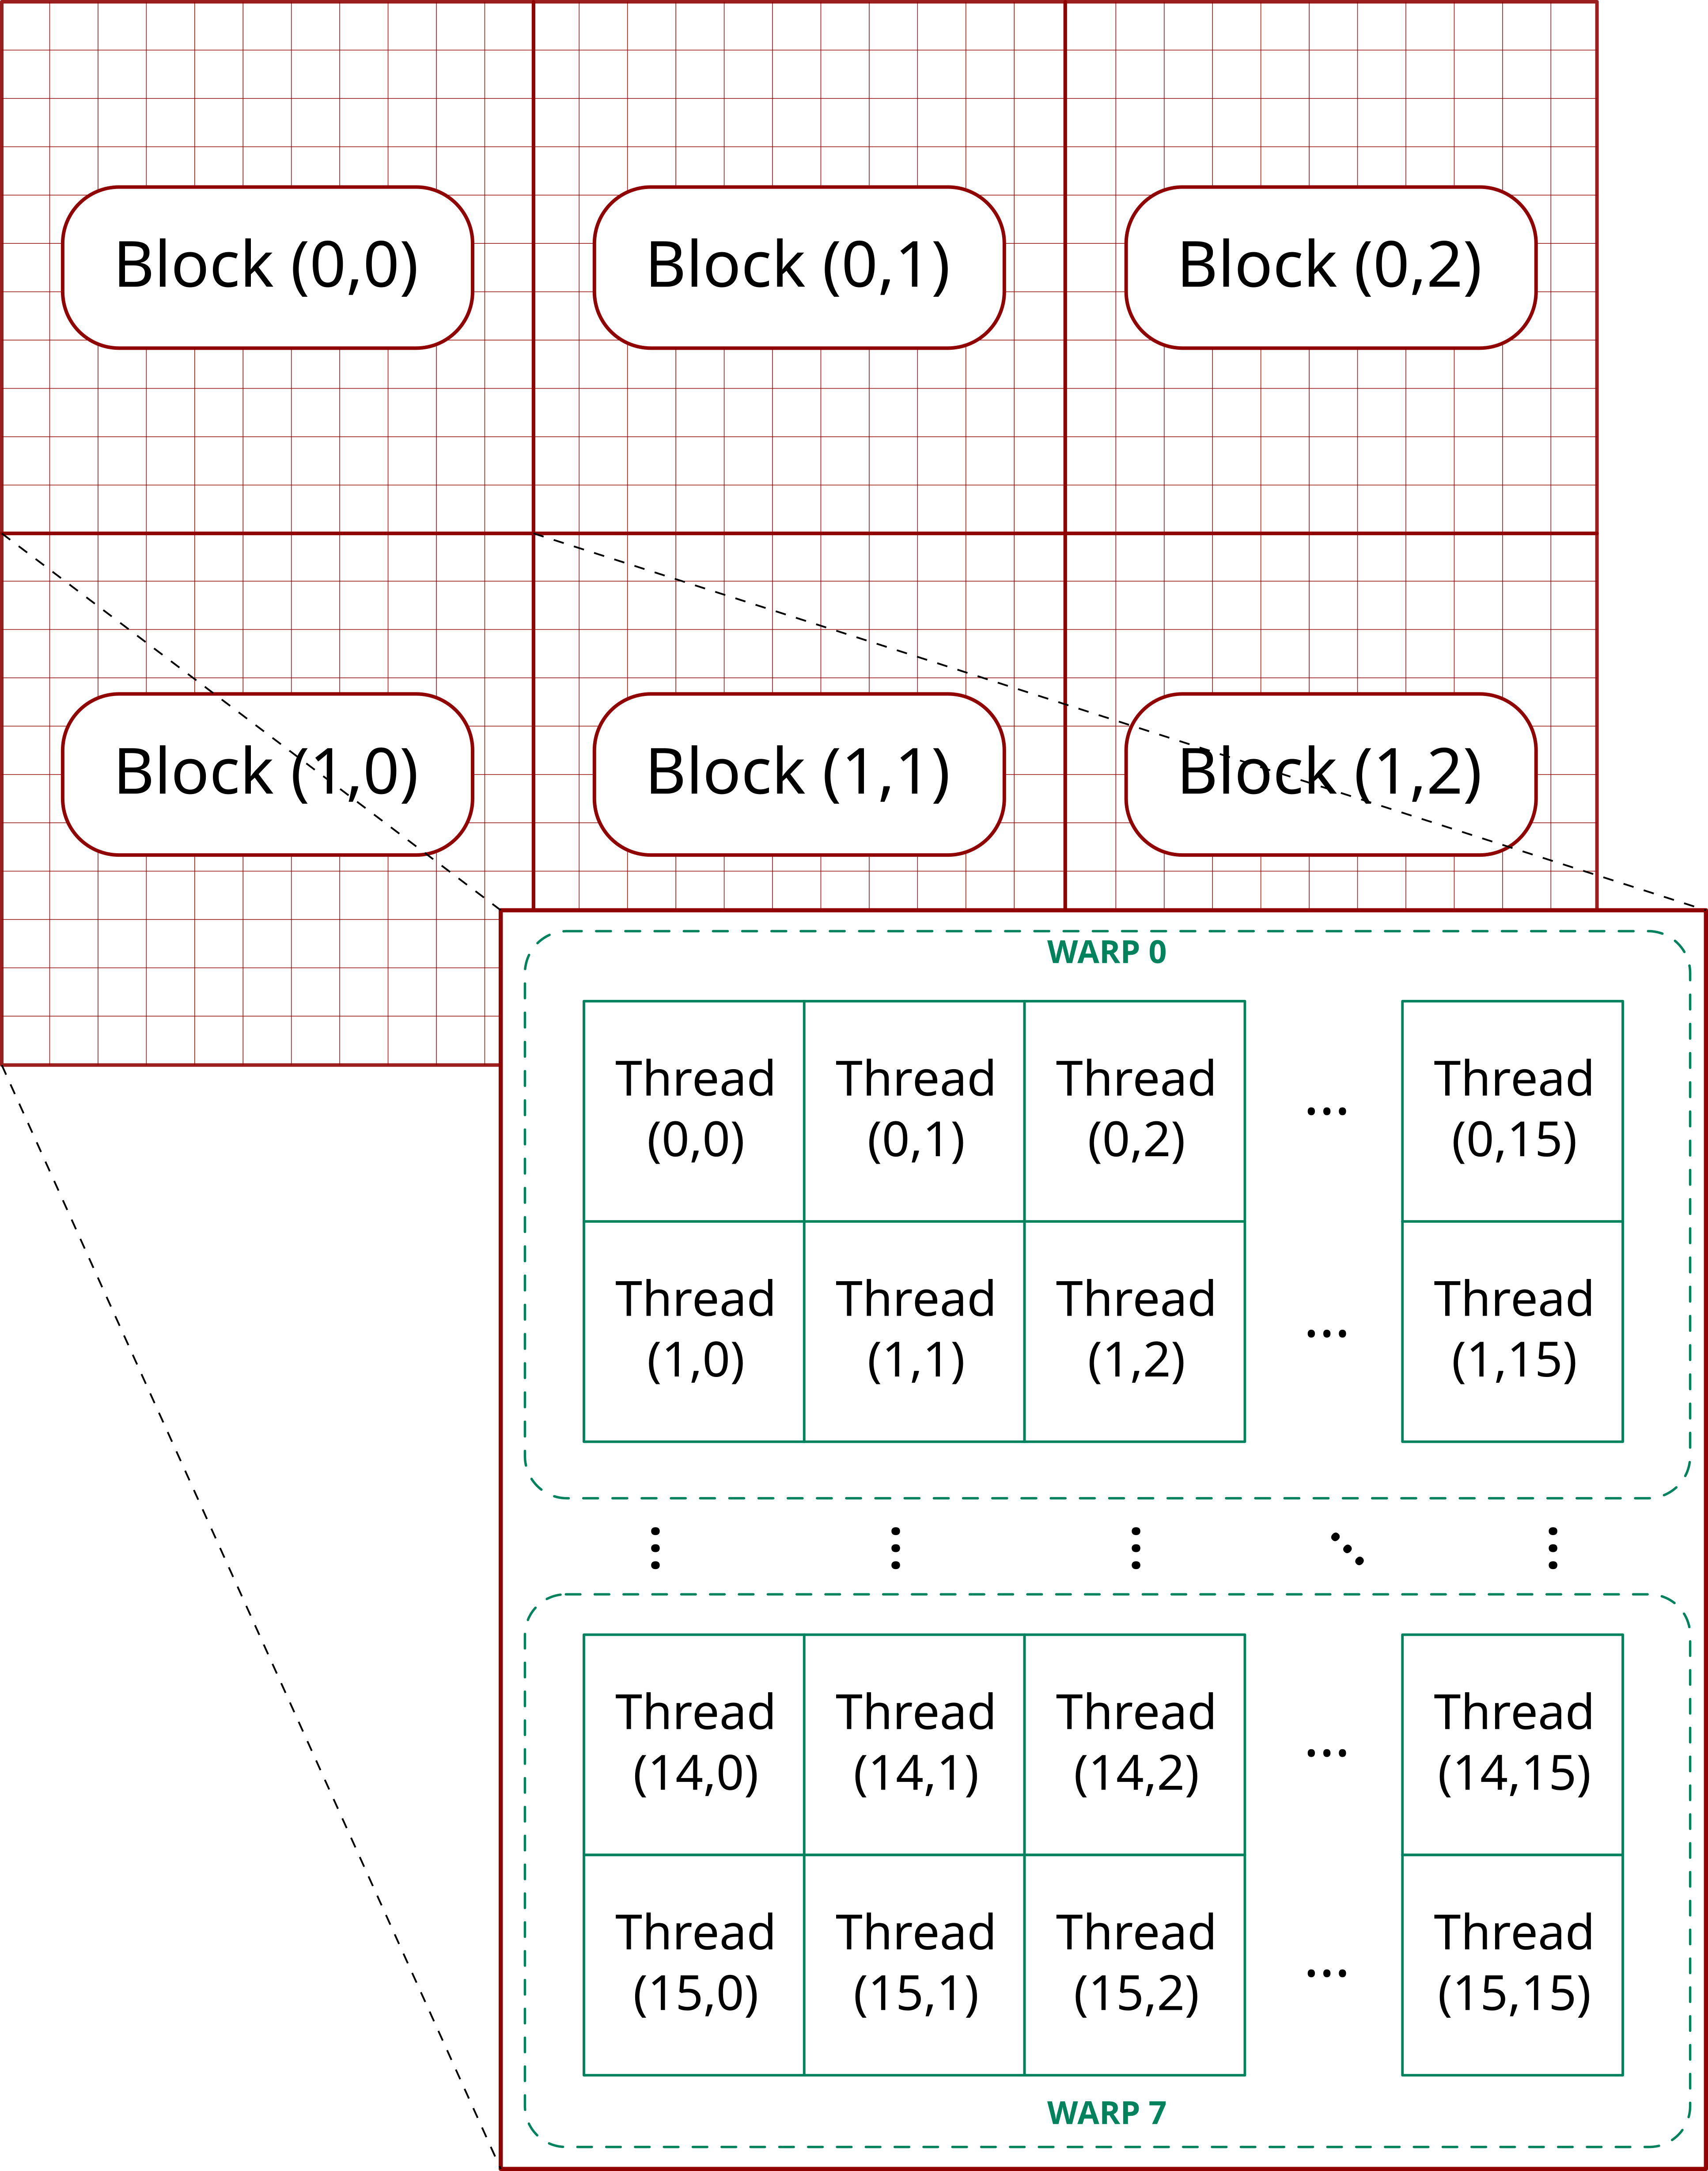
\includegraphics[width=.8\linewidth]{gfx/cudagrid.png}
	\caption[$2\times3$ grid with $16\times16$ blocks]{$2\times3$ grid with $16\times16$ blocks}
	\label{fig:cudagrid}
\end{figure}

An example configuration of the \ac{CUDA} device can be seen on \autoref{fig:cudagrid}, where 6 two dimensional blocks are arranged on the grid in two rows and three columns. Every block has 256 threads, arranged on a 16$\times$16 matrix.

The shape of the \ac{CUDA} grid and blocks are customizable by the user, but the warps are automatically created by \ac{CUDA}, picking up always sets of successive 32 threads, going first through the $X$ axis, then through the $Y$ axis and finally through the $Z$ axis.

This section will study how the grid and blocks are shaped on our software and the implemented parallelized code, as well as some fine-tuning techniques used to speed up the computations.

\subsection{Device Setup}
\subsection{CUDA Kernel}
\subsection{Fine-Tuning}